\documentclass[a4j,10pt]{jsarticle}
\usepackage{layout,url,resume}
\usepackage[dvipdfmx]{graphicx}
\pagestyle{empty}

\begin{document}
%\layout

\title{機械化された審判の導入}

% 和文著者名
\author{
    NECO B1 kosuke(渡辺孝亮) 
    \and
    親:ks91 }

% 和文概要
\begin{abstract}
現在のスポーツ界では、審判に人間を用いている競技が多々ある。本研究の目的は人間の審判を排除し、代わりに機械の審判を導入する事によって選手の誤審によるストレスを軽減することである。今回はテニスを具体例に、どのようなシステムをどのように導入すればよいかについて研究した。
\end{abstract}

\maketitle
\thispagestyle{empty}

\section{はじめに}

今日の世界では、さまざまなところで機械が活躍し、人間よりも正確で効率の良い仕事を行っている。これからはますます機械を用いる場所が増えていくと考えられる。しかし、スポーツの審判の世界ではいまだに人間が審判の役割を担っている。人間は機械に比べて、どうしてもミス・誤審の数・公平性に欠ける機会が多くなってしまう。誤審はプレーしている選手にとって精神面で大きなストレスとなり、選手が試合で本来の実力を発揮できなくなる原因となる可能性が非常に高い。
本研究ではテニスを具体例として、どのようなシステムをどのように導入すれば一般の人も手軽にしようでき、選手の負担を軽減することで現状よりも良い環境を提供することができるのかについて考察した。


\section{背景}

\subsection{現状のテニスのシステム}
現在テニスの公式試合は、主審と呼ばれる審判1名・先進と呼ばれる審判9名の計10人がコートを囲うように配置されボールがいんかアウトかを判定している。選手がその判定に納得できない場合には、”チャレンジシステム”によりセット内で3回のみ機械によって記録されたるリプレーを確認できる。



\subsection{ホークアイ}
先ほどのチャレンジシステムで用いられているのが、“ホークアイ”という機械である。
\\ 主に、
\begin{itemize}
\item ボールトラッキング
\item ビデオリプレイ技術を活用したCG画像のテクノロジー
\end{itemize}

を使用して、コートを囲うように設置されている複数台のカメラから、ボールとラインの関係をCGで映し出すことができる。
%---------------------------------------------

\section{仮説}
ホークアイを用いている現状のシステムでは、プロ選手などの限られた選手のみがその技術を利用することができ、多くの一般人は導入することが難しいと考えられる。そのため、この技術をより簡潔化した方法で利用することが必要である。
\section{実験}
\subsection{実験手法}
まずは現状のシステムに近いものに触れることが必要であると考えたため、ボールをトラッキングすることを試みた。今回はOpenCVというトラッキングシステムを用いて実験を試みた。
\\手法としては以下のようである
\begin{itemize}
\item フレーム間の差分画像を生成
\item 画像を2値化
\item 膨張処理して分割してしまった物体を1つの物体としてまとめる
\item 物体の重心座標(x,y)を計算し、円で囲う
\end{itemize}

\subsection{実験結果}

実験結果の画像を図1に示す。

\begin{figure}[htbp]
    \begin{center}
        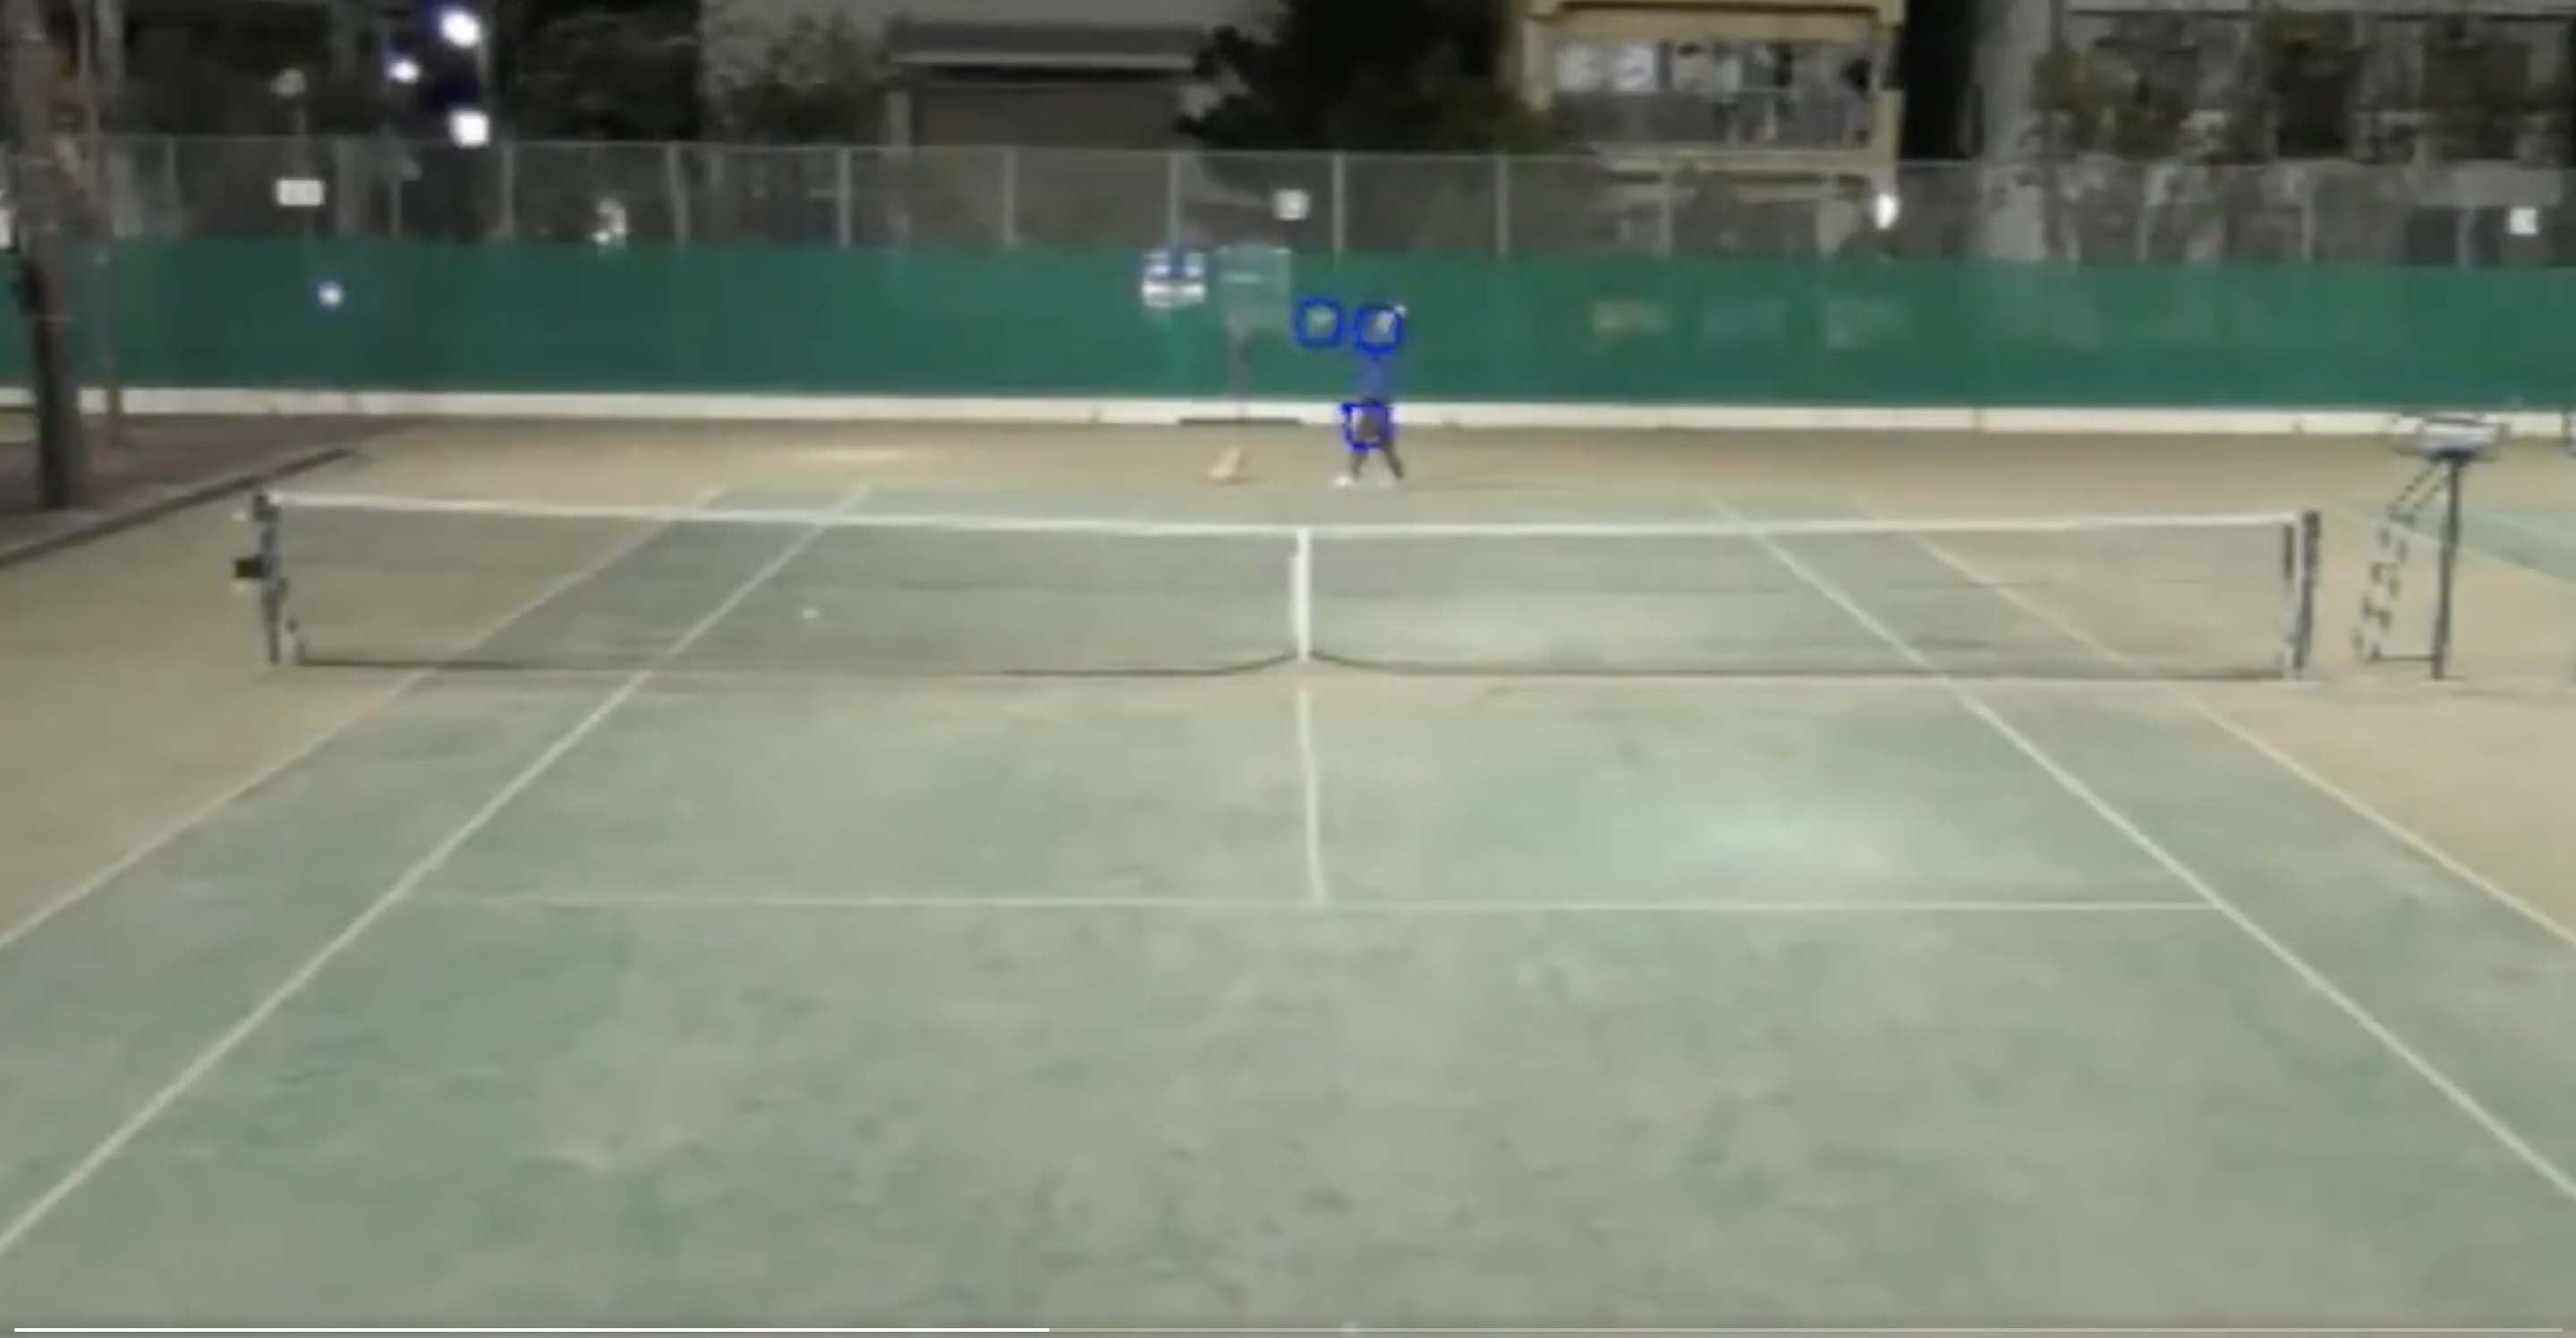
\includegraphics[width=6cm]{figure.png}
        \caption{ボールの位置を青丸により検出}
        \label{sample}
    \end{center}
\end{figure}
ボールの位置を検出することができたが、動くものに反応するため人など他のノイズも同時に検出してしまった。また、映像を用意してその解析を行うという手法をとるため、試合中にリアルタイムで表示することが難しく、また一般の人の利用も難しいを考えられる。
解像度についても十分とは言えず、より正確に映し出すことが必要であった。そのため、トラッキングシステムでは研究目的である試合を機械のみで運用すること、一般の人が手軽に使用できるという点を満たすことができなかったため改良が必要である。

\section{導入方法と倫理的問題}

全ての人間の審判を排除し、機械のみで公式試合を進行する事に対して倫理的な面から選手や学者から否定的な意見が多かった。過去に実験的にホークアイのみでテニスの試合を行ったことがあった。審判が目に入らないことで試合に集中できたという選手がいた一方で、人間→機械といういわば“上訴”のようなシステムがなくなってしまったことで信憑性が失われたという選手や、機械であれ2ミリから3ミリの誤差が生じているにも関わらず盲目的に信じてしまっているのはおかしいという学者もいた~\cite{hantei}~\cite{teku}~\cite{sport}。
\\競技は変わってしまうが、日本の国技である相撲は1969年にビデオ判定を導入した。これは他の競技と比べても非常に速く、導入当初は「伝統に科学を持ち込むのは良くない」という声が多く上がり、現在でも現在、ビデオ判定と土俵下の審判の意見が分かれた際は、人間の審判に権限がある事になっている。誰かが独裁的な権限を持つのではなく審判・行司・ビデオ判定員が集まり議論することが大切となっている~\cite{sumou}。
\\これは相撲に限らず全ての競技で言えることであり、ここに人間の存在意義が生まれてくるのではないかと考えた。形式上ではあっても機械は人間の手のひらの上で活躍すべきであり全ての進行を機械のみで行うのではなく人間と共生すべきであることがわかった。


\section{今後の展望}
今回はボールのトラッキングに焦点を当てて実験、研究したがこの手法ではどのように運用しても現状のシステムとあまり変わらず、リアルタイムで確認することが難しかった。また手軽に一般の人が利用することができないため別の方法を導入する必要がある。今後は、コートをスキャンなどする事ができる機械を提案し調査していきたい。それをネットに取り付けるなどしてリアルタイムで判定することができるようなものについて研究してゆく。アウトの時は赤、インの時は緑に光るなどの技術を利用すればプレーヤーにわかりやすく伝えることができるのではないだろうか。また、この技術をどのように応用すればテニス以外のスポーツに導入でき、人間と共生できるのかについても研究することが必要である。



%.........................
\begin{thebibliography}{99}
\bibitem{hantei} “判定者について: 審判と判定テクノロジーをめぐる社会学的考察” 柏 原 全 孝 
 追手門学院大学社会学部紀要 2015年3月30日,第9号,1-15 
\bibitem{teku} “正しい判定を作り出すテクノロジー” 柏原 全孝 
 スポーツ社会学研究 / 日本スポーツ社会学会 編, 第2号, 9-23, 1993
\bibitem{sport}“スポーツとテクノロジー:ホークア イシステムの場合” 柏原 全孝 
 甲南女子大学研究紀要, 人間科学編(54), 145-154, 2017 
\bibitem{sumou}“大相撲のビデオ判定前史-1950 年代のテレビ中継“ (柏原全孝)
\end{thebibliography}

\end{document}

% end of file
